\section{Preliminaries on TFHE}
\label{sec:preliminaries}



\subsection{Notations}

Let $\T = \R/\Z$ be the real torus, that is to say the additive group of real numbers modulo $1$. In practice, torus elements are not represented with an infinite number of digits, but are discretized. Let us denote this precision in base 2 as $\Omega$. We can define the discretized torus $\T_q = \{\frac a q \mid a \in \Z_q\}$ (the elements of the torus up to $\Omega$ bits of precision, $q$ being $2^\Omega$) and identify it with the ring $\Z_q$. As a consequence, any element $\frac a q$ of $\T_q$ will be represented in machine by $a$ without any loss of property of the group $\T_q$. The operations of sum $+$ and external product $\cdot$ have to be understood modulo $q$.

Moreover, for a natural integer $N$ and a given $q$, we will denote by $\T_{N, q}[X]$ the ring of polynomial $\T_q[X]/(X^N + 1)$. The elements of this ring are polynomials of maximum degree $N-1$ and with coefficients in $\T_q$. Like for the scalar version, this ring will be identified with the ring $\Z_q/(X^N + 1)$. $N$ is usually taken as a power of two.

Finally, we will denote by $\B$ the set of binary digits $\{0, 1\}$.  $\&$ and $\oplus$ denote the \texttt{AND} and \texttt{XOR} binary operations. For $x$ and $q \in \Z$ , $[x]_q$ denotes the reduction of $x$ modulo $q$. For $S$ a set, $x \drawfrom S$ denotes a uniformly random sampling from the set. For $\chi$ a distribution, $x \drawfrom \chi$ denotes a  random sampling according to the distribution.


\subsection{Complexity Assumptions}
\label{sec:complexity}

The TFHE scheme, as other schemes using lattices, relies on the hardness of the \LWE assumption. More precisely, it relies on the torus-based version of the problem. In the following, we consider the classic definition but over a discretized torus and with a binary secret:


\begin{definition}
    (\LWE problem over the discretized torus). Let $q, n \in \N$ and let $\vec s = (s_1, \dots, s_n) \drawfrom \B^n$. Let $\chi$ be an error distribution over $\Z_q$. The \emph{decisional Learning With Errors over discretized torus problem} is to distinguish samples chosen with the following distributions:
    
         \[\mathcal{D}_0 = \{(\vec a, r)\mid\vec a \drawfrom \T_q^n, r \drawfrom \T_q\}\]
    and:
         \[\mathcal{D}_1 = \{(\vec a, b)\mid\vec a = (a_1, \dots, a_n) \drawfrom \T_q^n, e \drawfrom \chi, b = \sum_{j=1}^n a_j \cdot s_j + e\}\]
    
    The \emph{search} version of the problem is to recover $\vec s$ from the samples of $\mathcal{D}_1$. 
    \label{def:LWE}
    \end{definition}


Both the search and decisional problems are reducible to each other \cite{Regev-LWE} and their average case is as hard as worst-case lattice problems.

\cite{TCHES:Joye22} argues that identifying the discretized torus $\T_q$ as $\Z_q$ makes the \LWE assumption over the discretized torus as hard as the standard \LWE assumption.


TFHE relies as well on the generalized version of \LWE over rings introduced in \cite{ITCS:BraGenVai12} named \GLWE.

\begin{definition}
    (\GLWE problem over the discretized torus). Let $N, q, k \in \N$ with $N$ a power of two and let $\vec s = (s_1, \dots, s_k) \drawfrom \B_N[X]^k$. Let $\chi$ be an error distribution over $\Z_{N, q}[X]$. The \emph{General decisional Learning With Errors over discretized torus problem} is to distinguish samples chosen with the following distributions:
        \[\mathcal{D}_0 = \{(\vec a, r) \mid \vec a \drawfrom \T_{N, q}[X]^k, r \drawfrom \T_{N, q}[X]\}\]
    and:
        \[\mathcal{D}_1 = \{(\vec a, b) \mid \vec a = (a_1, \dots, a_k) \drawfrom \T_{N, q}[X]^k, e \drawfrom \chi, b = \sum_{j=1}^k a_j \cdot s_j + e\}\]
    \label{def:GLWE}
    The \emph{search} version is analogous to the \LWE one.
\end{definition}
Note that \RLWE is simply an instantiation of \GLWE with $k = 1$.

The complexity analysis is analogous to the \LWE version.
In practice, the error distribution $\chi$ is a centered Gaussian distribution parametrized by its standard deviation $\sigma$.


\subsection{Plaintext Space}
\label{sec:plaintext_space}

\begin{wrapfigure}{r}{6cm}
    \centering
    \caption{Embedding of $\Z_p$ in $\Z_q$ \label{fig:embedding}}
    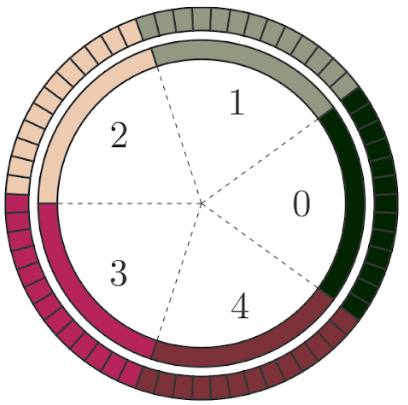
\includegraphics[width=5.5cm]{images/embedding.png}
\end{wrapfigure} 

Before expliciting more in depth the TFHE scheme, it is useful to define the \emph{plaintext space} and how it is embedded in the discretized torus. 

The plaintext space is the ring $\Z_p$, with $p \in \N$. For now, let us assume that $p \mid q$ and identify $\Z_p$ with $\T_p$. As $p \mid q$, all elements of $\T_p$ are elements of $\T_q$ as well. Thus, we can define a mapping $\rho: \Z_p \to \Z_q$ as $\rho: m  \mapsto \frac{m q} {p}$. 


Of course, only $p$ elements of $\Z_q$ are reached by such a mapping and they have the form $\left \{ \frac {k q}{p} \mid k \in \Z_p \right \}$. As they are evenly distributed across $\Z_q$, they define what we call \emph{sectors of $\Z_q$} of the form: 
\[\left \{ \left ( \frac{(2 k - 1)q}{2p}, \frac{(2k + 1)q}{2p} \right ) \mid k \in \Z_p \right \} ~.\] The embedding of $\Z_p$ in $\Z_q$ is illustrated in Figure \ref{fig:embedding}.

During encryption of $m$, some small noise $e$ is drawn from a Gaussian distribution over $\Z_q$ and is added to $m$. As $e$ is small, the noisy message $m + e$ stays in the same sector as $m$ but while homomorphic operations are carried out, the noise grows and may overflow out of the sector. When decrypting, one recovers the sum of the expected result and some noise $m' + e'$. As long as $e' < \frac{q}{2p}$, the message $m'$ can be recovered by rounding to the closest center of sector.



In our work, we pick odd values for $p$. $q$ being a power of 2 in practice, it implies that $p$ does not divide $q$. This enables nice features explained in Section \ref{sec:TFHE_adaptation}. Consequently, the centers and the bounds of sectors are computed by rounding the fractions to the closest integers. In practice, $p$ is much smaller than $q$ ($p$ is restricted to a few bits, while $q$ typically equals $2^{32}$ or $2^{64}$), so this discrepancy makes this approximation sound. In the following, we will ignore this rounding.


\subsection{Ciphertexts Types and Basic Operations}

TFHE manipulates several different types of ciphertexts. In the following, we explain their structure:

\begin{itemize}
    \item \textbf{TLWE ciphertexts}: The message $m$ to be encrypted is encoded as an element of $\T_q$. A mask $\vec a = (a_1, \dots, a_n)$ is drawn uniformely from $\T_q^n$ and a noise error $e$ is sampled from $\chi$. Using the secret key $\sk = (s_1, \dots, s_n) \in \B^n$, the body of the ciphertext is defined by $b = \sum_{j = 1}^n a_j \cdot s_j + m + e$. Finally, the TLWE ciphertext is $c = (\vec a, b)$. The decryption is performed by calculating the \emph{phase}: $\phi(c) = b - \langle \vec a, \vec s \rangle = m + e$ and rounding to the closest center of sector.\\

    \item \textbf{TRLWE ciphertexts}: It has the same global structure as TLWE ones, except the mask $\vec a$ is sampled from $\T_{N, q}[X]^k$, the secret key from $\B[X]^k$ and the error from $\T_{N, q}[X]$.
    Some papers in the literature use the denomination TRLWE only if $k = 1$, and TGLWE otherwise. In this work, we do not make a difference between both cases.

\end{itemize}


During the bootstrapping phase presented in Section \ref{sec:bootstrapping}, another structure (the TRGSW ciphertext) is used but we do not mention it as we will not need it. More details about TRGSW can be found in \cite{TCHES:Joye22}.


Two basics homomorphic operations are straightforward with these two structures: the component-wise sum of two TLWE (resp. TRLWE) ciphertexts $c_1$ and $c_2$ produces a ciphertext $c_3$ encrypting the sum modulo $p$ of the two underlying messages $m_1$ and $m_2$. Moreover, the external product $\lambda \cdot c_1$ with $\lambda \in \Z$ also produces an encryption of the multiplication $[\lambda \cdot m_1]_p$.


In the framework introduced by this paper, the freshly encrypted ciphertexts are TLWE, as well as during homomorphic computations. We only manipulate TRLWE ciphertexts during the \texttt{BlindRotate} phase of the bootstrapping, presented in Section \ref{sec:bootstrapping}.

\subsection{TFHE programmable bootstrapping (PBS)}
\label{sec:bootstrapping}

As defined by Gentry in \cite{gentry}, the procedure of bootstrapping can be defined as the homomorphic evaluation of the decryption circuit. In the context of TFHE, the hardest part to compute is the rounding of the value to an element of $\T_p$ by removing the noise. To achieve this homomorphically, it uses four procedures called \texttt{ModulusSwitch}, \texttt{BlindRotate}, \texttt{SampleExtract} and \texttt{KeySwitch}.\\\\


\textbf{\texttt{ModulusSwitch}:} The high level idea starts by homomorphically computing the phase $\mu \in \Z_q$ and reducing it to $\Tilde{\mu} \in \Z_{2N}$ by computing $\Tilde{\mu} = \left \lfloor \frac{\mu \cdot 2N} {q} \right \rceil$. In practice $N$ takes values between $2^{10}$ and $2^{13}$ so the most significant bits carrying the true value modulo $p$ are preserved. \\\\

\textbf{\texttt{BlindRotate}:}  Then, for a polynomial $v(X) \in \Z_{N, q}[X]$, called the \emph{accumulator}, one homomorphically multiplies $v(X)$ by $X^{-\Tilde{\mu}}$ by \emph{blind rotation} which yields an encryption of the polynomial $v_{\Tilde{\mu}} + v_{\Tilde{\mu} + 1} X + \dots \in \Z_{N, q}[X]$. By defining $v_j:= \frac1p {\left \lfloor \frac{jp}{2N} \right \rceil}$ $\forall j$, the blind rotation shall output an encrypted version of the message in the zero-degree coefficient. We do not explain here how this polynomial multiplication occurs, the reader is referred to \cite{cryptoeprint:2018/421} for a more elaborated explanation. The procedure outputs a TRLWE ciphertext of dimension $k$ encrypting the polynomial $X^{-\Tilde{\mu}} \cdot v(X)$. Note that the quotient polynomial of the ring has degree $N$ but $\Tilde{\mu}$ lives in $\Z_{2N}$ so each coefficient of $v_i$ can be reached with a multiplication by $X^{-\Tilde{\mu}}$ \emph{and} by $X^{[N - \Tilde{\mu}]_{2N}}$. In the latter case, the coefficient $v_i$ gets negated because of the ring modulus $X^N + 1$: we will refer to this problem as the \emph{negacyclicity problem}. One way to prevent this issue is to ensure that the most significant bit of $\mu$ is fixed at $0$ \cite{TCHES:Joye22} but a recent work \cite{AC:CLOT21} proposes a more sophisticated way to solve this problem. In our case, we use a modified version of the accumulator detailed in Section \ref{sec:TFHE_adaptation}.
\\\\

\textbf{\texttt{SampleExtract}: } This step simply extracts the degree-zero coefficient of the previous polynomial. It takes as input the TRLWE ciphertext yielded by the \texttt{BlindRotate} step and outputs the TLWE ciphertext $c'$ encrypting the original message $m$. However, this ciphertext is not immediately available for either further homomorphic computations or decryption, because it has a length $kN + 1$ instead of $n + 1$ (and as a consequence is encrypted under a different TLWE key).
\\\\

\textbf{\texttt{KeySwitch}: }  The previous step outputs the right value, but encrypted under a different set of parameters i.e. $c' \in \Z_q^{kN+1}$ while we are looking for $c \in \Z_q^{n}$. The only thing left is to convert $c'$ to $c$, which requires \emph{key switching keys} constructed from the secret key \sk used at encryption. More details about this specific step can also be found in \cite{cryptoeprint:2018/421}.
\\\\

This ``bland'' procedure of bootstrapping simply refreshes the noise in the ciphertext to put it back at the ``initial level'', but can be very simply turned into a \emph{Programmable} bootstrapping. Specifically it can simultaneously evaluate homomorphically any function $f$ on the input. To achieve this, at the construction of the accumulator, the coefficient $v_j$ is replaced by their evaluation by the function $f(v_j)$. This feature is extremely powerful and is the core of the huge potential of TFHE.



\subsection{Basics on Boolean Functions and Boolean Circuits}
\label{sec:preliminaries_boolean}

In this paper, we focus on the evaluation of Boolean functions with TFHE. A Boolean function has the form $f: \B^\ell \longrightarrow \B$, with $\ell$ being called the \emph{arity} of the function. 

\begin{definition}
    
The Algebraic Normal Form (ANF) of a Boolean function $f: \{0,1\}^\ell \mapsto \{0,1\}$ is a polynomial expression in which each term corresponds to a specific input combination of $n$ variables. The ANF is defined as follows: \[f(x_1, x_2, \ldots, x_l) = a_0 \oplus a_1x_1 \oplus a_2x_2 \oplus \ldots \oplus a_{2^n-1}x_1x_2\ldots x_l\] \begin{align*}
\text{where: }a_0, a_1, a_2, \ldots, a_{2^\ell-1} & \in \{0,1\} \quad \text{are the Boolean coefficients and} \\
x_1, x_2, \ldots, x_\ell & \quad \text{are called the Boolean variables}
\end{align*}
\end{definition}

This result means that any Boolean function can be evaluated by the means of \texttt{AND} and \texttt{XOR} operations. In the following, we will focus on the implementation of Boolean circuits composed of these operations exclusively.


A Boolean function can be represented by its \emph{truth table}, which is simply a table gathering all the possible inputs and the corresponding result of the application by the function. It can also be represented with a Boolean formula. A third representation is the \emph{Boolean circuit}:

\begin{definition}
    A Boolean circuit associated to the Boolean function $f$ is a finite Directed Acyclic Graph whose edges are \emph{wires} and vertices are \emph{Boolean gates} representing Boolean operations. We consider \texttt{AND} gates and \texttt{XOR} gates, of fan-in 2 and fan-out 1. We also consider copy gates, of fan-in 1 and fan-out $>1$, that outputs several copies of its input. A circuit is further formally composed of input gates of fan-in 0 and fan-out 1, and output gates of fan-in 1 and fan-out 0.
    
    Evaluating a $\ell$-input $m$-output circuit consists in writing an input $\vec{x} \in \B^\ell$ in the input gates, processing the gates from input gates to output gates, then reading the outputs from the output gates.

\end{definition}


This notion of Boolean circuit will be particularly useful in Section \ref{sec:graphs}.

